\section{A Lesson Wrapped in an Illusion}
\label{SEC:background}


A magician creates an illusion to hide the secrets of his or her trick.
The lessons we have developed reverse this situation.
Instead of hiding secrets, we use our tricks to reveal
the mysteries behind
three cyberattacks.
Our tricks were chosen because of their relevance to the information
security field and, following the principles of scaffolding, are presented
in order of increasing technical complexity.
This section details how the mechanics of each trick mirror the
rationale behind the attacks by illustrating both the magician's and
participants' perspectives.  Video tutorials for each of the tricks are
available at: \textit{(URL removed for blinding purposes)}.

%We also include variations on each trick
%that can
%improve the
%trick's impact or make it easier to perform under certain circumstances.

%\subsection{Lesson Layout}
%
%For our lesson topics we decided on three topics: social engineering, side
%channel attacks, and attacks on randomness.
%These attacks were chosen
%because they
%are highly relevant to the modern information security field,
%and offer different levels of complexity.
%Our hope was to illustrate how card magic can be used
%successfully to teach anything from simple deceptive scenarios to complicated
%technical attacks.
%Following the principles of scaffolding,
%we chose to present the least technical attack -- social engineering --
%first.  This gives students something to build on when we introduce more
%difficult concepts.
%
%Section~\ref{SEC:evaluation} presents further information on how our lesson
%was presented as well as the instruments used to assess its effectiveness.

\subsection{Social Engineering}

In the context of information security,
"social engineering" is defined as a set
of tactics to manipulate users into giving away personal information.
We start with this attack as it is broadly used and affects arguably the
greatest cross-section of victims.  This portion of our demonstration
is a simulation of the attack because it is engineered to give
the magician multiple opportunities to ask for personal information,
such as a participant's full name or date of birth.
The magician employs two card tricks
as
both a misdirection and a cover
in order to
distract the
volunteer participant from
the true intention: soliciting
personal data that
can be used to compromise accounts,
reset passwords using security questions, or
carry out identity theft.

At the end of the trick, the magician reveals that this information
collection was the true purpose of the trick.
Examples of real world social engineering attacks round out the
presentation.

\subsubsection{From the Audience's Perspective}

Our version of this trick is adapted from a magic classic
known as ``The Red and Black Separation Trick~\cite{redblackseparation}.''
The magician begins by
telling the audience that there
is a way to form a psychic bond with a deck of cards
and requesting a student volunteer.
The volunteer and magician
together prepare the deck
by each shuffling half of the cards.
The two halves of the deck are then combined by placing one half
one on top of the other.
Next, the magician asks the volunteer
a few questions, starting with their birth year,
to allegedly further ``attune''
the link between the individual and the deck.
The response
is used to select one red card and one black card from the deck,
each with a numeric value equal to one of the last two digits of
the volunteer's birth year.
Next, the magician asks for the volunteer's birth month and similarly selects
a red card with a numeric value equal
to their birth month (using the jack and queen for November and December
respectively).
Finally, the magician asks
for their birthday and selects a black card with a numeric value
equal to the second digit in this day.
The magician lays these cards out on the table and asks the volunteer to select
one red card and one black card with which they feel most ``attuned''.
The unchosen cards are returned to the middle
of the deck face up.

At this point, the magician declares
that it is time to test the volunteer's psychic powers by asking them to
guess the color of each card in the deck.  Starting with the top of the deck,
the volunteer guesses either ``red'' or ``black,''  while the magician
places the card face down on top of the card of the same
color already on the table.
This forms two piles of cards.

Half-way through the deck,
the two face up cards are placed on top of the
pile of the opposite color, switching the color assignments of
each pile.
The volunteer continues guessing
with red cards going onto the new red pile and vice versa
until
there are no cards remaining.
At this point the magician turns over the face
down cards to reveal that the volunteer has correctly guessed {\textbf every}
card's color, building the illusion that a psychic connection has been made.

With the volunteer ``hooked,'' the magician keeps pumping for information by
suggesting the deck can read minds.
The deck is put back together
and the volunteer shuffles it
a few times before cutting it into two piles.
The magician
selects one of the piles and, without looking at it,
reveals the bottom card to the volunteer and the
audience.
This pile is placed on top of the other pile perpendicularly so that
the volunteer's card remains accessible.  The magician then asks the volunteer to
make a series of statement pairs with one being true and one being false.  For
example,  the magician may ask the volunteer to state  ``I was born in
\textit{blank},'' with blank being replaced by their birth city, and ``I was
born in Moscow, Russia,'' (assuming the volunteer was \textit{not} born in Moscow,
Russia).  A similar process is used to have the volunteer make true/false
statement pairs about where they attended school earlier in their life, the name
of their childhood best friend, and other similar details about their life.

After the magician has elicited a number of statements sufficient to
``hone in on the volunteer's psychic link,''
a second set of true/false statement pairs are used
to figure out the volunteer's card.  This is done by asking the volunteer to make
statement pairs like ``My card is red'' and ``My card is black.''  Similar
pairs regarding the card's suit and value allow the magician to zero
in on the volunteer's card.
At this point, the magician reveals that the volunteer had been
``misdirected'' into performing the tricks true purpose -- revealing
personal information.  This creates a teachable moment for discussing
the types of information that can be used in identity theft attempts
should they
be made public.


\subsubsection{Behind the Scenes}

\begin{figure}[H]
\centering
\includegraphics[scale=.6]{images/Trick1}
\caption{Arrangement of cards after participant has guessed the color of each
card in the deck.  The ``correct column'' contains the red cards in a red pile and
the black cards in a black pile.  The ``incorrect column'' contains the reverse.
Correct cards are revealed by flipping each pile in place.  Incorrect cards are
made to appear correct by using the discussed flipping technique.}
\label{fig:trick1}
\end{figure}

Before the trick begins, the deck has already
been separated into red and black halves.
The volunteer receives one of these halves,
meaning
the initial shuffling efforts are merely scrambling
cards of the same color.
Therefore, when the two packs are
stacked one on top of the other the two colors remain
separate.
The magician must make note of where in the deck
one color ends and the other begins.

In the first question and answer portion of the trick the magician is able to
pull out two red and two black cards that reflect the volunteer's answer.  The
volunteer then picks two of these cards to remain out while the other two are
returned to the deck.  The magician must return these cards face
up exactly between the red and black ``sections'' of the deck.
This is used in the next phase of the
trick to signal the magician when all of one color of card
has been dealt into one of the two piles.

During the prediction phase of the trick, the volunteer believes that they are
guessing the color of cards from a mixture of red and black.
In reality,
the volunteer is guessing all the cards of one color and then all cards of
the other.
This means for the first half of the deck, one pile contains all correct
guesses while the other is completely incorrect.
When the midway point is reached the magician takes the two face up cards and places the
red one face up on the black pile and vice versa.
This means that the ``correct'' pile will continue to accumulate correct
guesses and the ``incorrect'' pile incorrect ones.

After all the cards have been guessed, there will be two piles,
one containing all correct guesses and the other
all incorrect guesses.
An illustration of this arrangement appears in Figure~\ref{fig:trick1}.
The reveal proceeds as follows.
First, the magician shows that the volunteer accurately guessed all of the cards
in the correct pile by flipping the piles horizontally.
Next, the magician reveals the ``incorrect'' pile by collecting the
entire pile and flipping it forward vertically.  This
reverses the incorrect guesses so that the red cards are now paired
with the red marker card and the black with the black marker.  This completes
the illusion that the volunteer correctly guessed {\textbf every} card in the
deck.

To set up the second trick, the magician combines the piles and asks the
volunteer to shuffle them.  During this process, the magician must pay close
attention to which card appears on the bottom of the deck.  This is possible
because many novices reveal the faces of a deck when shuffling.  Next,
the magician asks the volunteer to cut the deck into two packs.  The pack that
formed the bottom of the deck pre-cut is placed perpendicularly on
top of the other, ensuring that the volunteer's card was the bottom card of
the deck pre-cut. Instead of simply revealing this information the
magician uses the statement pairs component of the trick to ``pump'' the volunteer
for more information.

%\subsubsection{Variations}
%
%...

\subsubsection{Lesson Takeaway}

This trick is intended to spark a teachable moment about
social engineering and
its dangers.
The most powerful point comes with the reveal that the magician's
intended goal was stealing personal information.
Building upon this reveal allows instructors to start a dialog with
students about what other
sorts of information attackers might try to steal and
how they could maliciously use it.
Having given the students a scaffold on which to build,
an instructor can
introduce a more formal definition of social engineering
and the aspects of human nature that allow such attacks to succeed.
The facilitator concludes with two real world examples --
social media ``quizzes'' and phishing campaigns.
Participants should walk away with a sense of the
dangers of social engineering and a tool-set they can use to protect
themselves and others.

\subsection{Side Channel Attacks}

As the name implies, a side channel attack strikes a target indirectly
by tracking seemingly unrelated phenomena
such as timing information, power consumption, electromagnetic leaks, or even
sounds.  To mirror this type of attack, the trick
demonstrates how an attacker can
gather information without directly exploiting
a vulnerability in a system or algorithm.
The main version of this trick enlists a ``side channel'' to
enable the magician to easily
find a particular card that has been lost in a shuffled deck.
For the card trick, the ``side channel'' comes from a variation on a magic
technique called ``marking the cards.''  Our trick works with a normal deck
of cards due to information on the printed pattern on the card back.  In a
sense, the card was already ``marked.''  The trick also borrows from a
group of tricks based on a card being upside-down in the deck.

\subsubsection{From the Audience's Perspective}

The magician begins by opening a new deck of cards, removing the jokers and
branding cards, and legitimately shuffling it.  Several volunteers are
asked to
select a card from the deck, show it to the audience, memorize it without
revealing it to the magician, and then return it to the deck.
The magician shuffles the deck a few more times ensuring that the cards
have
been completely lost.
It concludes with the magician going through the deck face down
until all of the volunteers' cards have been found.

This trick's reveal comes when the magician informs the audience
that the cards were found using a secret
information side channel present in the
deck and asks if they have any idea of what it might be.
At this point, the audience is either stumped or has figured out how the trick
worked.

In either case,  the second phase of the lesson
introduces additional types of side channels
by having an assistant
-- a ``stooge'' in magic terminology --
surreptitiously
communicate the details of a card
to the magician.
The assistant selects a card and asks the magician questions about its
attributes.
For example, ``Is my card red or black?''
When asking these questions the volunteer
telegraphs a response
by varying the pitch of their voice, vocal cadence, or body language.
After sufficient questioning, the magician is able to determine which card the
volunteer picked and asks the audience if they were able to determine the side
channel used to communicate this information.

\subsubsection{Behind the Scenes}

\begin{figure}[H]
\centering
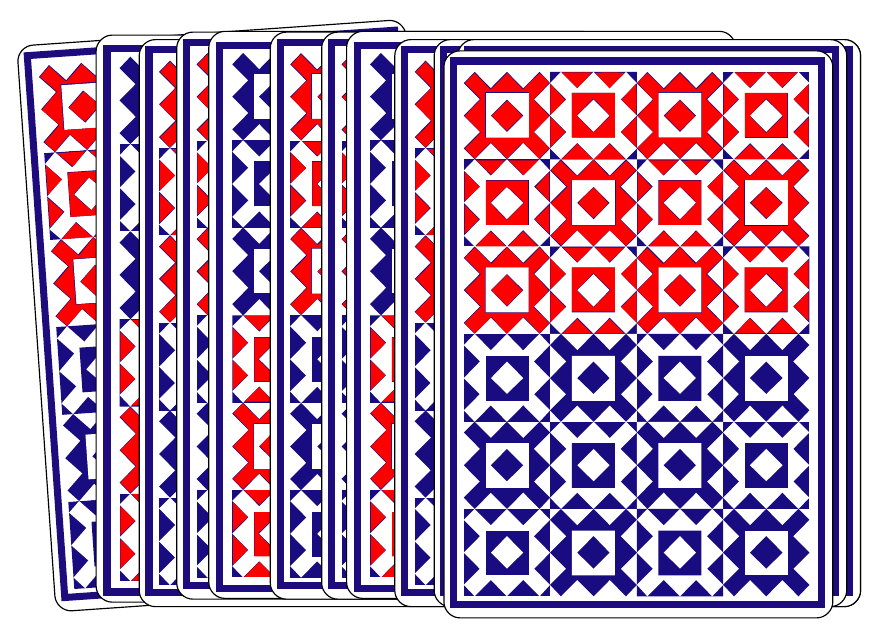
\includegraphics[scale=.7]{images/Trick2}
\caption{Flawed card backs allow the magician to see when a card is
``upside-down'' in the deck.  The magician takes advantage of this by
  turning cards upside-down when returning
  them to the deck after the participants have memorized them.}
\label{fig:trick2}
\end{figure}

The key to this trick lies in the magician's choice of deck.  Many cheaper card
decks, such as those given away as branded merchandise,
have corporate logos or
text on the card back.  Often, these patterns are used to
provide information about how a card is oriented in the deck.  Because the trick
begins with a fresh deck, all cards are oriented in the same direction.  As a
result, when the volunteer is returning their card to the deck, the magician
simply has to orient the deck in such a way that the volunteer's card is returned
in the opposite direction to the other cards.  During all shuffling
operations, the magician may maintain this orientation by rotating one pack of a
cut deck so that it's post-shuffle orientation matches the other pack.
To complete the trick, the magician only has to look through the deck of cards
and find the card with a differing orientation.  Figure~\ref{fig:trick2}
illustrates the magician's view of the deck of cards before the trick's
reveal.

%\subsubsection{Variations}
%
%...

\subsubsection{Lesson Takeaway}

Side channel attacks are not easily spotted.  Our goal is to
open the participant's eyes to less
obvious avenues an attacker might use.
The reveal of this trick shows how we must not
take anything at face value, including what information
a card can contain.
Subtle details of the graphics on its back and even its orientation in a
deck enable the magician to identify a card, just as physical phenomena,
such as temperature, sound, and even electromagnetic output can
leak private data.
This provided a framework
to discuss side channels
as a security weakness that allows information to
be extracted via attributes
of a system, rather than a flaw in an
algorithm.
In order to emphasize the impact of such attacks we cover two examples: Van
Eck Phreaking and the SPECTRE vulnerabilities.
The former is a technique where images displayed by a computer monitor can be
detected and reconstructed using off-the-shelf radio hardware.
The latter is a major vulnerability recently discovered in many popular
types of
processors that uses timing information to extract sensitive data from a
computer's memory.
The lesson concludes with tips on how to
reduce the risk of a side channel attack
by minimizing the number of potential channels,
and actively working to decouple potential
side channels from secret information.

\subsection{Attacks on Randomness}


True randomness is important in many
security-sensitive situations.
An attacker who is able to predict or influence the output of a random number
generator may use this capability to circumvent cryptographic security controls.
The trick we use to cover this concept
illustrates a potential vulnerability in cryptographic hash functions
-- that the last input to the function has a high degree of control over
the function's output.

Our trick relies on a foundational technique called ``forcing a card,''
defined as a ``a method of controlling a choice made by a spectator during
a trick~\cite{forcingcard}.''
In this case, the forcing relies on how the card in question is positioned
in the deck, how the deck is shuffled, and the magician's control over the
random number generator.

\subsubsection{From the Audience's Perspective}

The trick begins with the magician announcing that it is possible to
guess the value of a card that
has been randomly selected from the deck.
The magician
explains that this is possible because every
card has different amounts of ink on its face.
This gives each card
a unique
weight that can be detected by feel.
To prove this point,
The magician spreads a deck of cards on the table face up
in order to prove its authenticity,
shuffles the deck,
and deals five cards out on the table.
The magician will make a prediction from these cards.
In order to head off suspicion that sleight of hand has been used to ensure
a specific card made it into the candidate set, the magician reveals that
a software random number generator will be used to select the card to be
guessed.
Students are asked to shout out numbers to be fed into the random number
generator to seed its operation.  After many numbers have been input, the
magician generates a number between 1 and 5, with each value referring to a
specific card.  The magician moves the chosen card forward and slides it back
and forth on the table to get an idea of its weight.  The magician then makes
a prediction and reveals that it is correct!

\subsubsection{Behind the Scenes}

\begin{figure}[H]
\centering
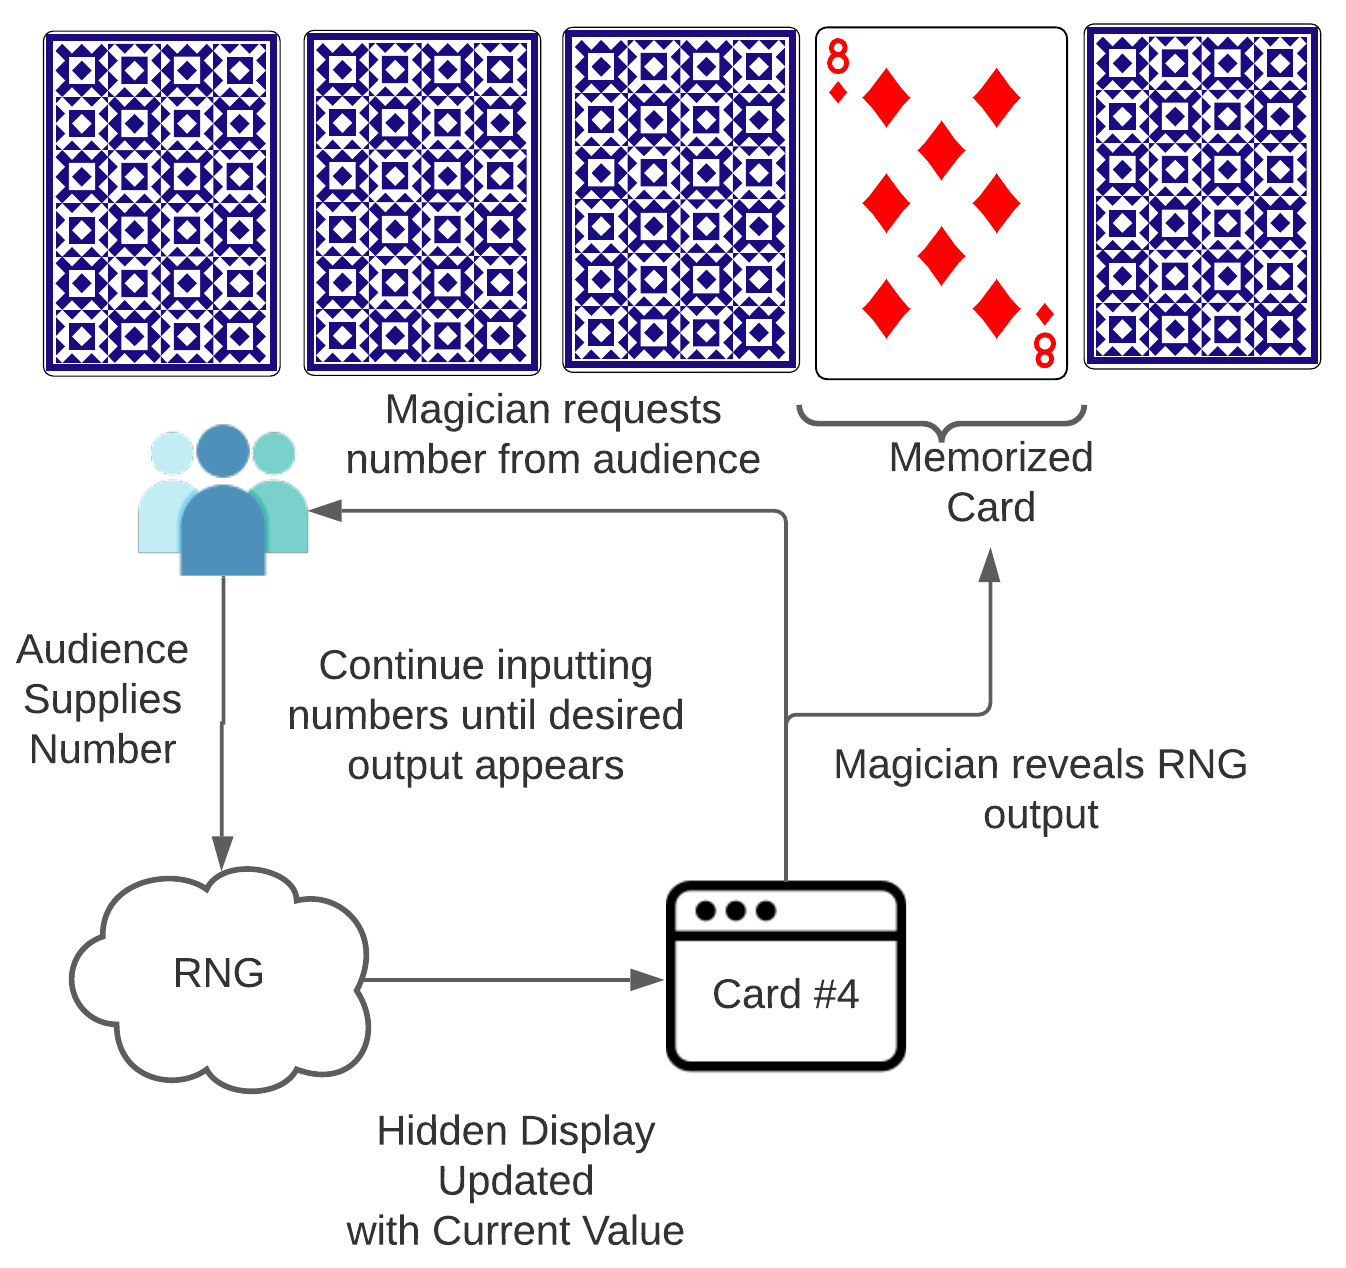
\includegraphics[scale=.6]{images/Trick3}
\caption{Participant inputs are repeatedly fed into our ``random number
generator'' in order to seed its output.  The magician stops entering inputs
when a hidden display indicates a memorized card would be chosen.}
\label{fig:trick3}
\end{figure}

The success of this trick relies on two elements.
The first is when the deck is spread out on the
table before the students.  This movement serves the dual purpose of convincing
the students that the deck is genuine and gives the magician a chance to
memorize one or more of the top five cards in the deck.
When the deck is
shuffled, the magician is careful to not allow the cards that were memorized to
become mixed in with the rest of the deck.  This is easily accomplished by
using a standard riffle shuffle and ensuring that the top several cards of
the deck are allowed to fall as a unit after the remainder of the deck has
been shuffled normally~\cite{wikishuffle}.
Keeping the top of the deck intact allows them to ensure that
these cards will be dealt onto the table prior to making a prediction.


The second key lies in how the random number is generated.
Rather than
a true software random number generator, the magician's tool is based on a hash
function.  This means that, while output appears random, it is anything but.
As students' shouted numbers are fed into the tool the magician monitors an
intermediate output.
This output shows the result of first feeding a student's number
into the hash function, then using modulus to reduce the output to a value
between zero and four, and finally adding one in order to get a value between
one and five.
The magician can use this input to determine when the output will be a number
corresponding with a card they have memorized and stop supplying inputs.
Figure~\ref{fig:trick3} illustrates how these two pieces interact to make
the trick work.


%\subsubsection{Variations}
%
%...

\subsubsection{Lesson Takeaway}

The purpose of this lesson is to show students the importance of correct
randomness
that is "fit for purpose," or appropriate for security-sensitive applications.
It also shows how an attacker
with a small amount of influence,
such as when to stop supplying numbers,
can compromise a
system.
As such, we begin by covering the common pitfalls
that occur when generating and
using randomness.
This foundation is used to explain both
direct and input-based attacks on random
number generators.
The explanation of these attacks gives our students the background they need to
understand why the magician's random number generator was invalid as well as
many of the most important properties of cryptographic hash functions.

%The trick we use reinforces this using
%a situation where ``users'' are able to provide input
%directly to a cryptographic hash function.
%We build on this by discussing how these functions work and their importance
%in applications like cryptocurrency and password storage.
